\documentclass[
    parskip=half, 
    twoside=false,
    twocolumn=true,
    fontsize=11pt,
]{scrarticle}
\usepackage{xcolor}
\definecolor{seeblau}{HTML}{00A9E0}
\definecolor{seegrau}{HTML}{9AA0A7}

\definecolor{seeblau1}{HTML}{CCEEF9}
\definecolor{seeblau2}{HTML}{A6E1F4}
\definecolor{seeblau3}{HTML}{59C7EB}
\definecolor{seeblau4}{HTML}{00A9E0}
\definecolor{seeblau5}{HTML}{008ECE}


\usepackage{graphicx}
\usepackage{amsmath}
\usepackage{subcaption}
\usepackage{wrapfig}
\usepackage[english]{babel}
\usepackage{blindtext}
\usepackage{microtype}
\usepackage{siunitx}
\usepackage[utf8]{inputenc}
\usepackage{csquotes}
\usepackage{nicefrac}
\usepackage[T1]{fontenc}
\usepackage{amsfonts}
\usepackage{amssymb}
\usepackage{tikz}

\usepackage{siunitx}

\usepackage{libertinus, libertinust1math}
\usepackage{roboto}

\setkomafont{disposition}{\normalfont\sffamily}


% not recommended with KOMA-script
% make table of contents sans-serif
% \usepackage{tocloft}
% \renewcommand\cftchappagefont{\normalfont}
% \renewcommand\cftchapfont{\normalfont}
% \renewcommand\cftchappresnum{\bfseries}
% \renewcommand\cftchapaftersnum{}
% \renewcommand{\cftchapfont}{\sffamily}
% \renewcommand{\cftsecfont}{\sffamily}
% \renewcommand{\cftsubsecfont}{\sffamily}
% \renewcommand{\cftchappagefont}{\sffamily}
% \renewcommand{\cftsecpagefont}{\sffamily}
% \renewcommand{\cftsubsecpagefont}{\sffamily}

% caption
\usepackage{caption}
\captionsetup{
	% font={sf},
	labelfont={sf, bf, color=seeblau},
	labelsep=quad,
	labelformat=simple,
}

% links
\usepackage{hyperref}
\hypersetup{
	colorlinks=true,
	linkcolor=seeblau,
	citecolor=seeblau,
	urlcolor=seeblau,
	% hidelinks=true
}

% bibliography
\usepackage[
	style=numeric-comp, % comp = compressed 4,5,6,7 -> 4-7
	sorting=none,		% Sort by appearance
	% autocite = superscript,
	% backref=true,
	hyperref=true,
	url=true,
	maxbibnames=100
]{biblatex}
\DefineBibliographyStrings{english}{%
    backrefpage  = {see p.}, % for single page number
    backrefpages = {see pp.} % for multiple page numbers
}

% remove issue
\AtEveryBibitem{%
  \clearfield{number}
}

\usepackage{float}
% \floatplacement{figure}{h}
% \floatplacement{table}{H}

% loosen float placement rules
\renewcommand{\topfraction}{0.8}
\renewcommand{\bottomfraction}{.8}
\renewcommand{\textfraction}{0.1}
\renewcommand{\floatpagefraction}{.9}
% make floats less likely to be placed on a separate page
\setcounter{totalnumber}{9}
\setcounter{topnumber}{9}
\setcounter{bottomnumber}{9}

% decrease space between floats and text
\setlength{\textfloatsep}{0.5cm}
\setlength{\floatsep}{0.5cm}


\usepackage{adjustbox}

\usepackage{datetime}
\newdateformat{dotdate}{
	\twodigit{\THEDAY}.\twodigit{\THEMONTH}.\THEYEAR
}
\newdateformat{monthyeardate}{%
  \monthname[\THEMONTH] \THEYEAR}


% header and footer
\usepackage[
  markcase=noupper
]{scrlayer-scrpage}% activates pagestyle scrheadings automatically
\clearpairofpagestyles
\setkomafont{pageheadfoot}{\normalfont\sffamily}
\setkomafont{pagenumber}{\normalfont\sffamily}
% \chead*{\color{seegrau} Draft \dotdate\today}
\ofoot*{\pagemark}
\ohead*{\rightmark}


\usepackage{ifthen}
\newcommand{\markieren}[4]{
    \ifthenelse{\equal{#1}{}}{}{\adjustbox{padding=3pt, bgcolor=seeblau1, margin=-1pt}{\strut{\sffamily\robotoMedium{#1}}}\\}
    \ifthenelse{\equal{#2}{}}{}{\adjustbox{padding=3pt, bgcolor=seeblau2, margin=-1pt}{\strut{\sffamily\robotoMedium{#2}}}\\}
	\ifthenelse{\equal{#3}{}}{}{\adjustbox{padding=3pt, bgcolor=seeblau3, margin=-1pt}{\strut{\sffamily\robotoMedium{#3}}}\\}
	\ifthenelse{\equal{#4}{}}{}{\adjustbox{padding=3pt, bgcolor=seeblau4, margin=-1pt}{\strut{\sffamily\robotoMedium{#4}}}}
}

\addbibresource{literature.bib}

\begin{document}

\title{title}
\subtitle{subtitle}
\author{Aurel Müller-Schoenau, Leon Oleschko}
\date{\dotdate\today}


% make a custom title page
\begin{titlepage}
    \sffamily
    \vspace*{3cm}
    {
        \fontsize{32}{32}
        \markieren{}{}{}{Motencarlo}
    }
    \vspace{.25cm}\\
    {
        \Large
        Aurel Müller-Schoenau, Leon Oleschko\\
        Supervised by Philipp Baumgärtel
        \vspace{.05cm}\\
        22.01.2025
        \vspace{.25cm}\\
        \normalsize
        Physikalisches Fortgeschrittenenpraktikum 2\\
        Universität Konstanz
    }
    \vfill
    {
        \normalfont\normalsize
        TODO
    }
    \vfill
    \begin{flushright}
        Available at \url{www.github.com/leoole100/fp2}.
    \end{flushright}
\end{titlepage}

\section{Introduction}
In physics research we ususally try to rely on very simplified model systems. This lets us investigate dynamics deterministically under controlled conditions to analyse each and every relevant interplay. However, nature is complex and modeling real systems may lead to the question - How do you analyse systems so complex they have a (practically) indefinite amount of degrees of freedom?\\
Statistical physics deals with this issue by making assumptions based on the idea that nature approaches thermodynamic equilibrium. This simplifies the dynamics of a single particle because one may assume the interactions with the rest of the system can be reduced to random interactions following a certain distribution. Computer-based methods making use of random numbers as means for simulation are generally called \textit{Monte-Carlo-Methods}.\\
In this experiment, we simulate the one-dimensional trajectory of a particle inside different energy potential landscapes under the influence of random kicks. Our goal is to confirm the theoretical models derived in statistical mechanics.

\section{Results}
\subsection{Free Particle}
\begin{figure}
\label{fig:pt1_trajectory}
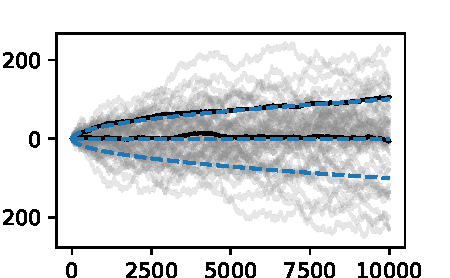
\includegraphics{figures/01 time trace.pdf}
\end{figure}
\begin{figure}
\label{fig:pt1_msd}
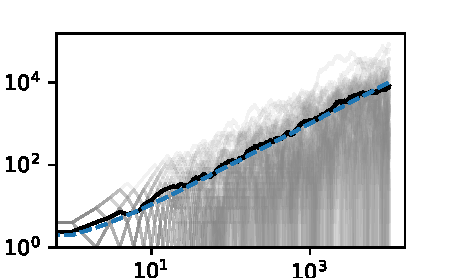
\includegraphics{figures/01 msd.pdf}
\end{figure}

% TODO: Diagramme: Trajektorien, Mean Trajectorien, MSQ mit theoretischer Kurve

In the first part of this experiment, the simple goal was to get a simulation running with nothing more than a freely moving particle in one dimension. The code was written in python and parallelised using NumPy. The trajectory was initialised at position \SI{0}{}. For each timestep, a displacement of $\Delta x_n \in \{\pm \Delta x\}$ was applied in either the positive or negative direction, chosen randomly (at each timestep) with equal probability. This results in Brownian Motion shown in \autoref{fig:pt1_trajectory}. Simulation data was generated for \SI{50} individual trajectories, each one being simulated for a total of $N=\SI{10000}{}$ timesteps. The expected result are freely diffusive dynamics, as shown in the plot. The \textit{Mean Square Displacement} is defined by
\begin{equation}
 MSQ(t_n) = x^2(t_n), \qquad t_n = n \cdot \Delta t
\end{equation}
Since the displacements for different timesteps $t_i\neq t_j$ are uncorrelated, we expect that
\begin{align}
 MSQ(t_n = n \Delta t) &= \left(\sum_{i=1}^n \Delta x_i\right)^2 \\&= 2 \cdot \underbrace{\sum_{i<j\leq n} \Delta x_i \Delta x_j}_{=0} + \sum_{i=1}^n \Delta x_i^2 \\ &= n \cdot \Delta x^2
\end{align}
The MSQ averaged over all \SI{50}{} trajectories is shown in \autoref{fig:pt1_msd} alongside the theoretical prediction.


\subsection{Potential Well}
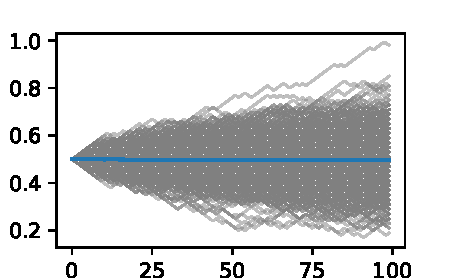
\includegraphics{figures/02 time evolution.pdf}

\subsection{Harmonic Potential}

\subsection{Double Well}


\pagebreak
\section{Conclusion}


\addcontentsline{toc}{section}{Literature}
\nocite{*}
\printbibliography

\end{document}
